\documentclass[a4paper,aps,prl,12pt,tightenlines,superscriptaddress]{revtex4}
\usepackage[top=72pt, bottom=72pt, left=72pt, right=72pt]{geometry}

\usepackage{natbib}
\usepackage{multirow}
\usepackage{graphicx}
\usepackage{tipa}
\usepackage{marvosym}
\usepackage{color}
\usepackage{placeins}
\usepackage{tabularx, ragged2e,booktabs, caption}
\usepackage[top=1in,
bottom=1in,
left=1in,
right=1in]{geometry}

\newcommand{\noteme}[1]{\noindent \textbf{[[JCW:  #1 ]]}}

\title{}
%\author{}
%\date{}

\begin{document}

\begin{center} \textbf{Allophonic Emergence: three ways allophonic rules come to be} 
 \end{center}

%\maketitle


We are now reaching the point in the fields of language change, sociolinguistics, and language acquisition where we can go well beyond Neogrammarian descriptions of sound change, and even beyond the influential work by Kiparsky \noteme{get refs}, to ask nuanced questions about how phonological systems emerge. This is to say that we can now treat the ``actuation problem'' as more than just a problem \citep{wlh1968}: it is a research program, with hypotheses posed at a high level of detail. In this paper, we consider the actuation of allophonic splits. \textcolor{blue}{(something about yay corpus data?)}

We argue that there are three distinct possible diachronic paths to allophony, all of which may be currently attested:

\textbf{Mechanical Means:} The traditionally assumed scenario, recently elaborated by Burmudez-Otero \noteme{get refs}: a low-level phonetic, articulatory, or acoustic/perceptual effect created by a phonotactic context becomes strong enough to be phonologized, reanalyzed at some point by learners as an allophonic rule. 

Info about aspiration in NW England English. 

\textbf{Spontaneous phonologization:} Speakers spontaneously create an allophone without any phonetic motivation: speakers split one phonological category into two through a pure reanalysis, creating an allophone with no initial phonetic difference from the other allophone. Subsequently, over generational time, the two purely phonological allophones diverge phonetically. Fruehwald (2013) provides an example of spontaneous phonologization in the \textsc{price} split in Philadelphia, providing evidence that the reanalysis of pre-voiceless \textsc{price} and pre-elsewhere \textsc{pride} preceded \textsc{price}-raising in the community.

%\floatbarrier
\textbf{Phonological Specialization:} %A purely phonetic change begins, creating variation in phonetic space, and then different sections of this variation begin to specialize for different phonological contexts over time. The phonological change occurs as a reanalysis of the ``old'' and ``new'' variants of a phonetic change in progress, after that change is well underway (for independent reasons). 
A purely phonetic change begins, creating variation in phonetic space. This variation become reanalyzed as distinct allophonic variants for a given generation of speakers. We see an example of allophonic specialization in \textsc{goose}-fronting in New Zealand English, with \textsc{goose} beginning to front as a single variant which then splits into preceding yod \textsc{new} and non-yod \textsc{goose} words (see Figure 1). We argue that this is distinct from the traditionally mechanical means of allophonic split in production as well as in the predictions about possible conditioning environments.

\begin{figure}
\begin{center}
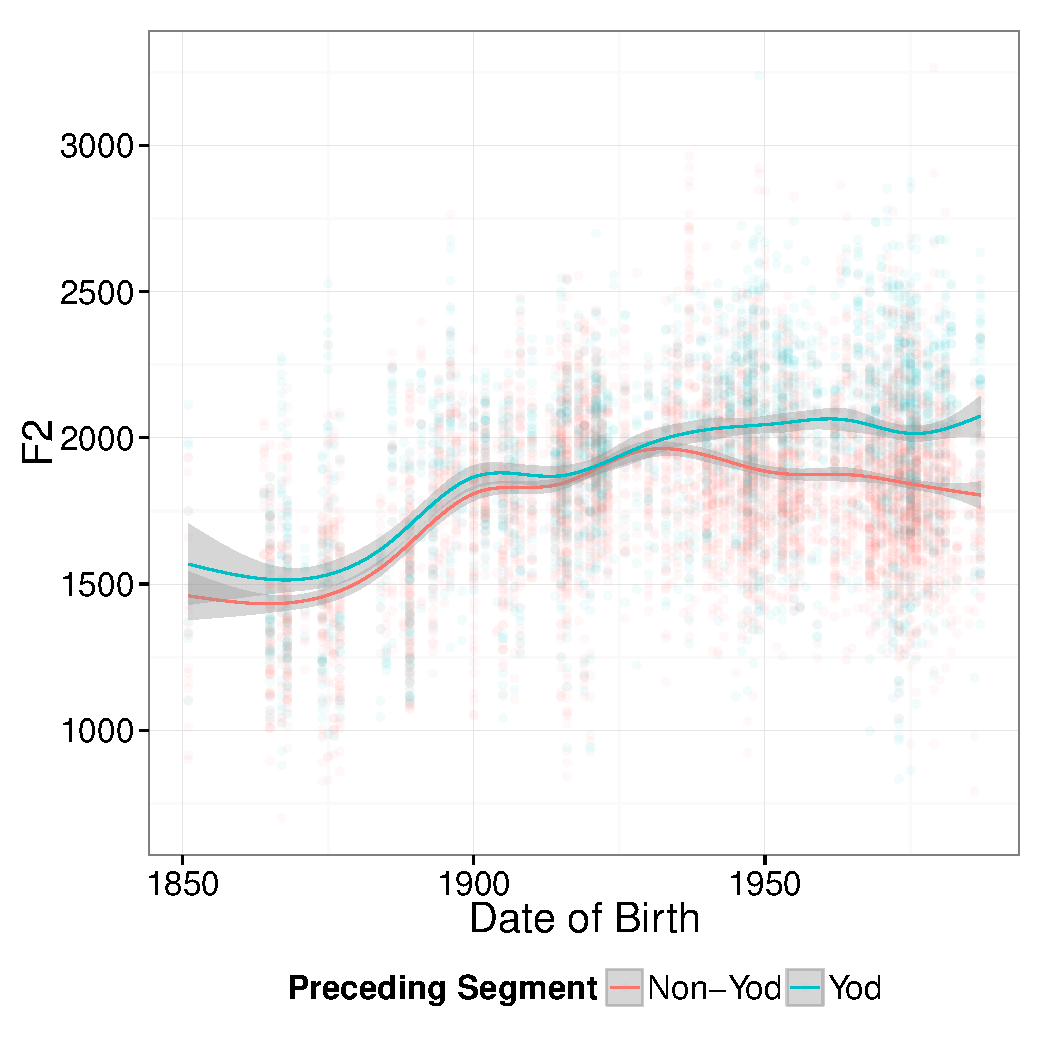
\includegraphics[width=.5\textwidth]{ByTokenOldPreceding.pdf}
\end{center}
\caption{stuff}
\label{newzeaFig}
\end{figure}

%\floatbarrier

\noindent Each of these three pathways to allophonic split make distinct predictions about the production \textcolor{blue}{(and perception?)} of the variants involved. We present evidence suggesting that all of these scenarios have occurred in the histories of languages, and suggest a research program to distinguish these three scenarios in production data. 

%Rather, we intend to present discussion as a challenge to the fields of historical phonology and sociolinguistics to either confirm or falsify these hypotheses, or to show that some of these scenarios can in fact be reduced to one of the others. 

references

\end{document}